\chapter{Results}\label{ch:results}

The results from both a simulation in MATLAB and a simulation on the actual helicopter are presented here.


\section{Helicopter simulation in MATLAB}

The plots from the simulation in MATLAB are presented here. 


Below are plots of the helicopter equations simulated in MATLAB.

The system is simulated with a generated disturbance sequence, which is described in section \ref{sec:methodology}. The values are $10 \: deg \leq w \leq 12\:  deg.$


The finite horizon for the \acrshort{mpc} is $N = 15$.

First, the simulation without a terminal cost or terminal constraint.

\begin{figure}[h!]
    \centering
    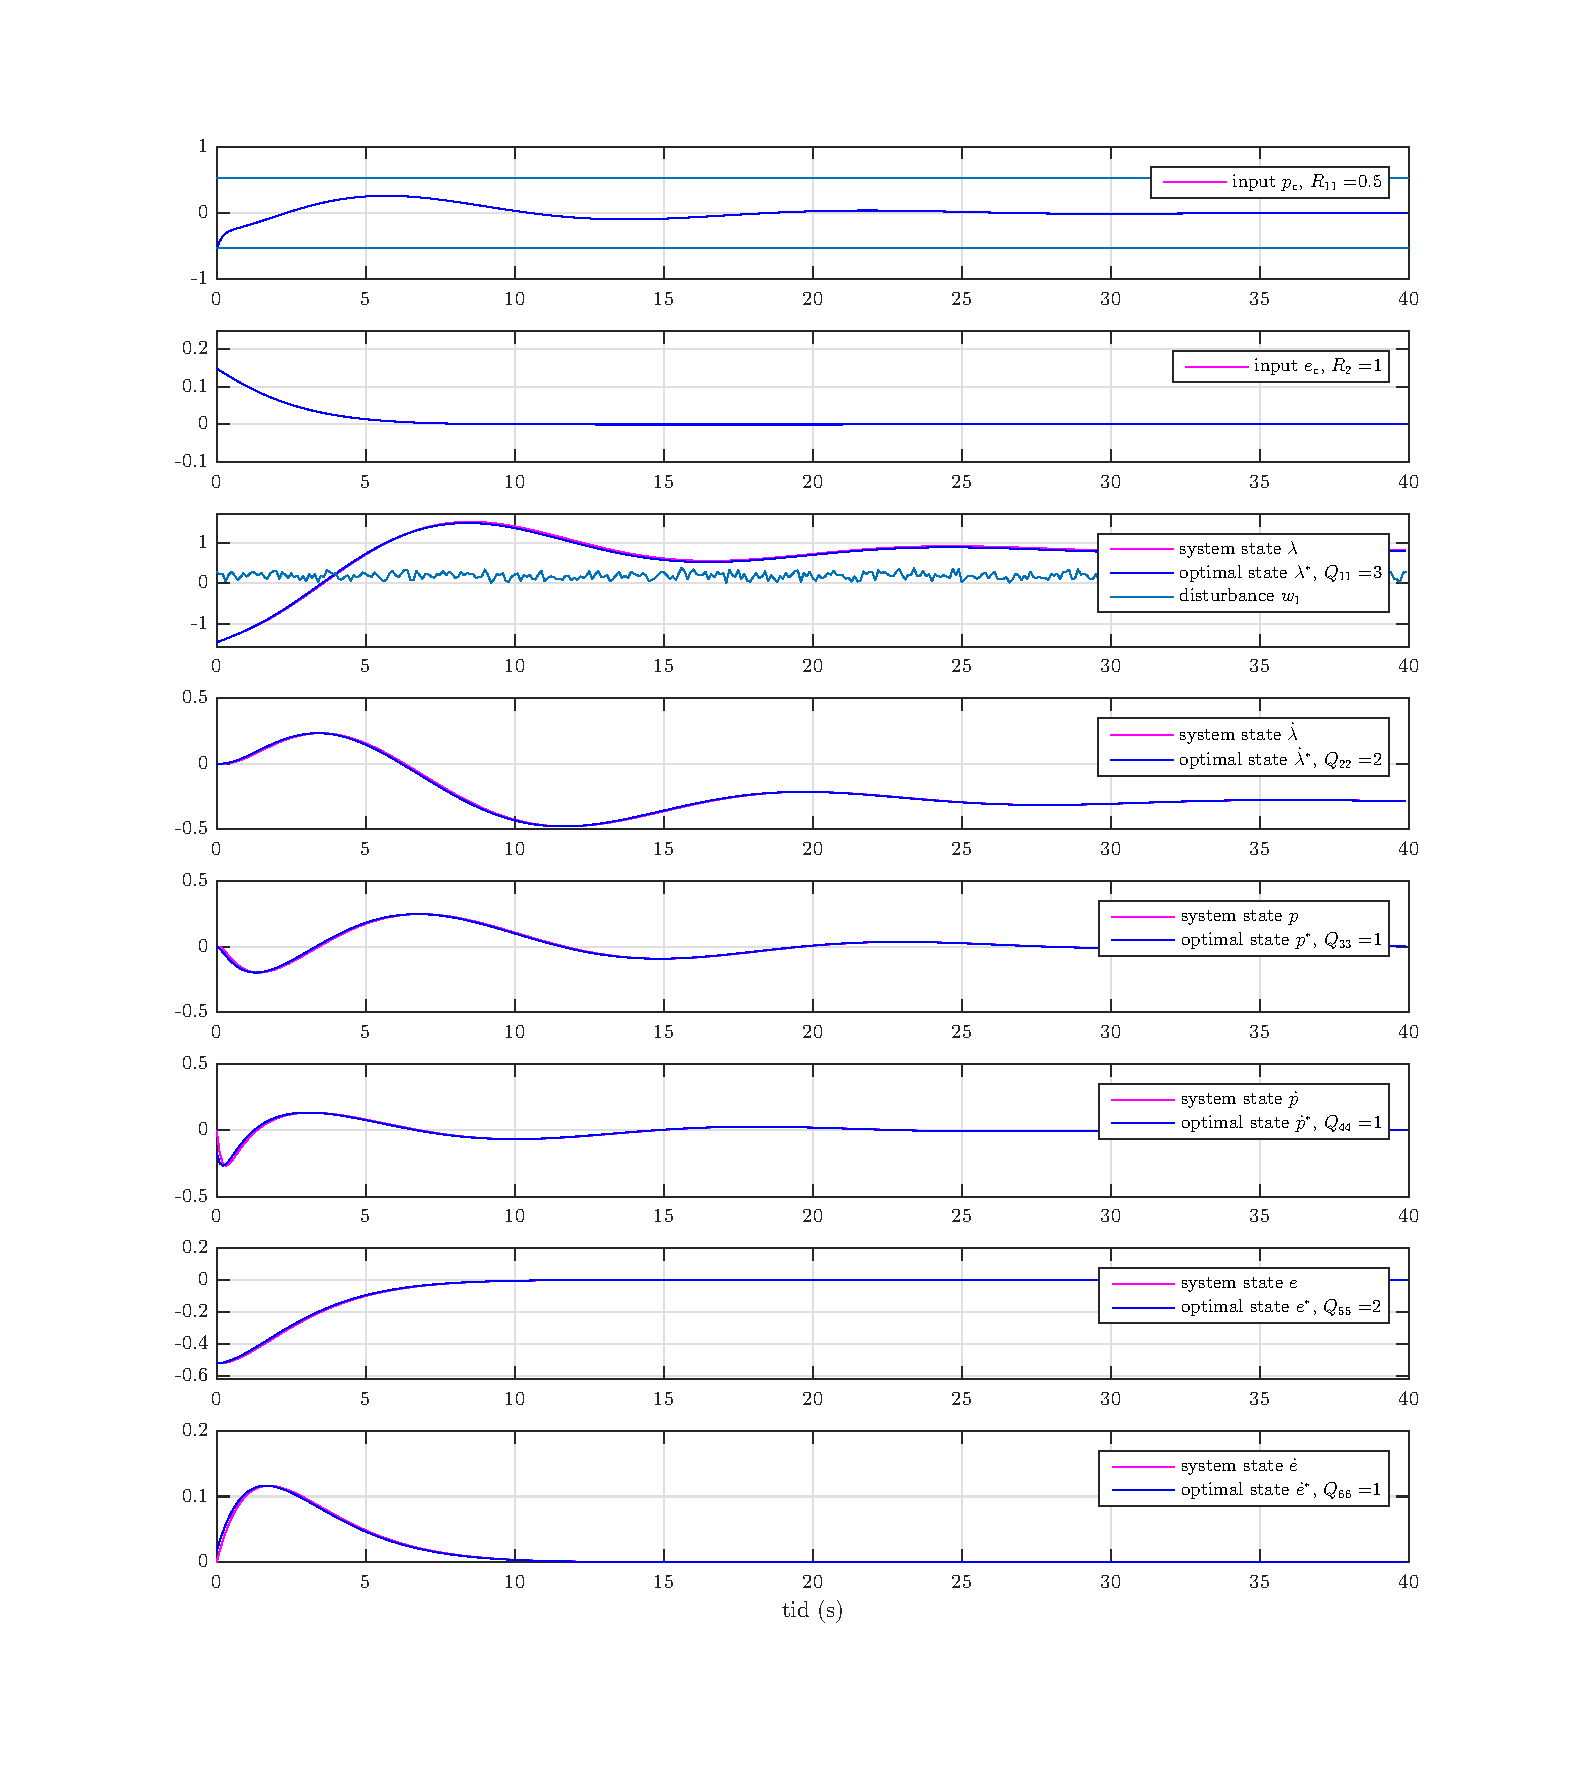
\includegraphics[scale=0.4]{fig/heli_sim_no_est_not_stable_extended_horizon.eps}
    \caption{Simulation in MATLAB with nominal \acrshort{mpc}}
    \label{fig:my_label}
\end{figure}

The travel $\lambda$, after 30 seconds, varies between $[0.7778, 0.8282]$. 

Further, the estimator described in section \ref{sec:estimator} is implemented. The goal is to model the disturbance applied, to try to remove the constant deviation in $\lambda$. 

\begin{figure}[h!]
    \centering
    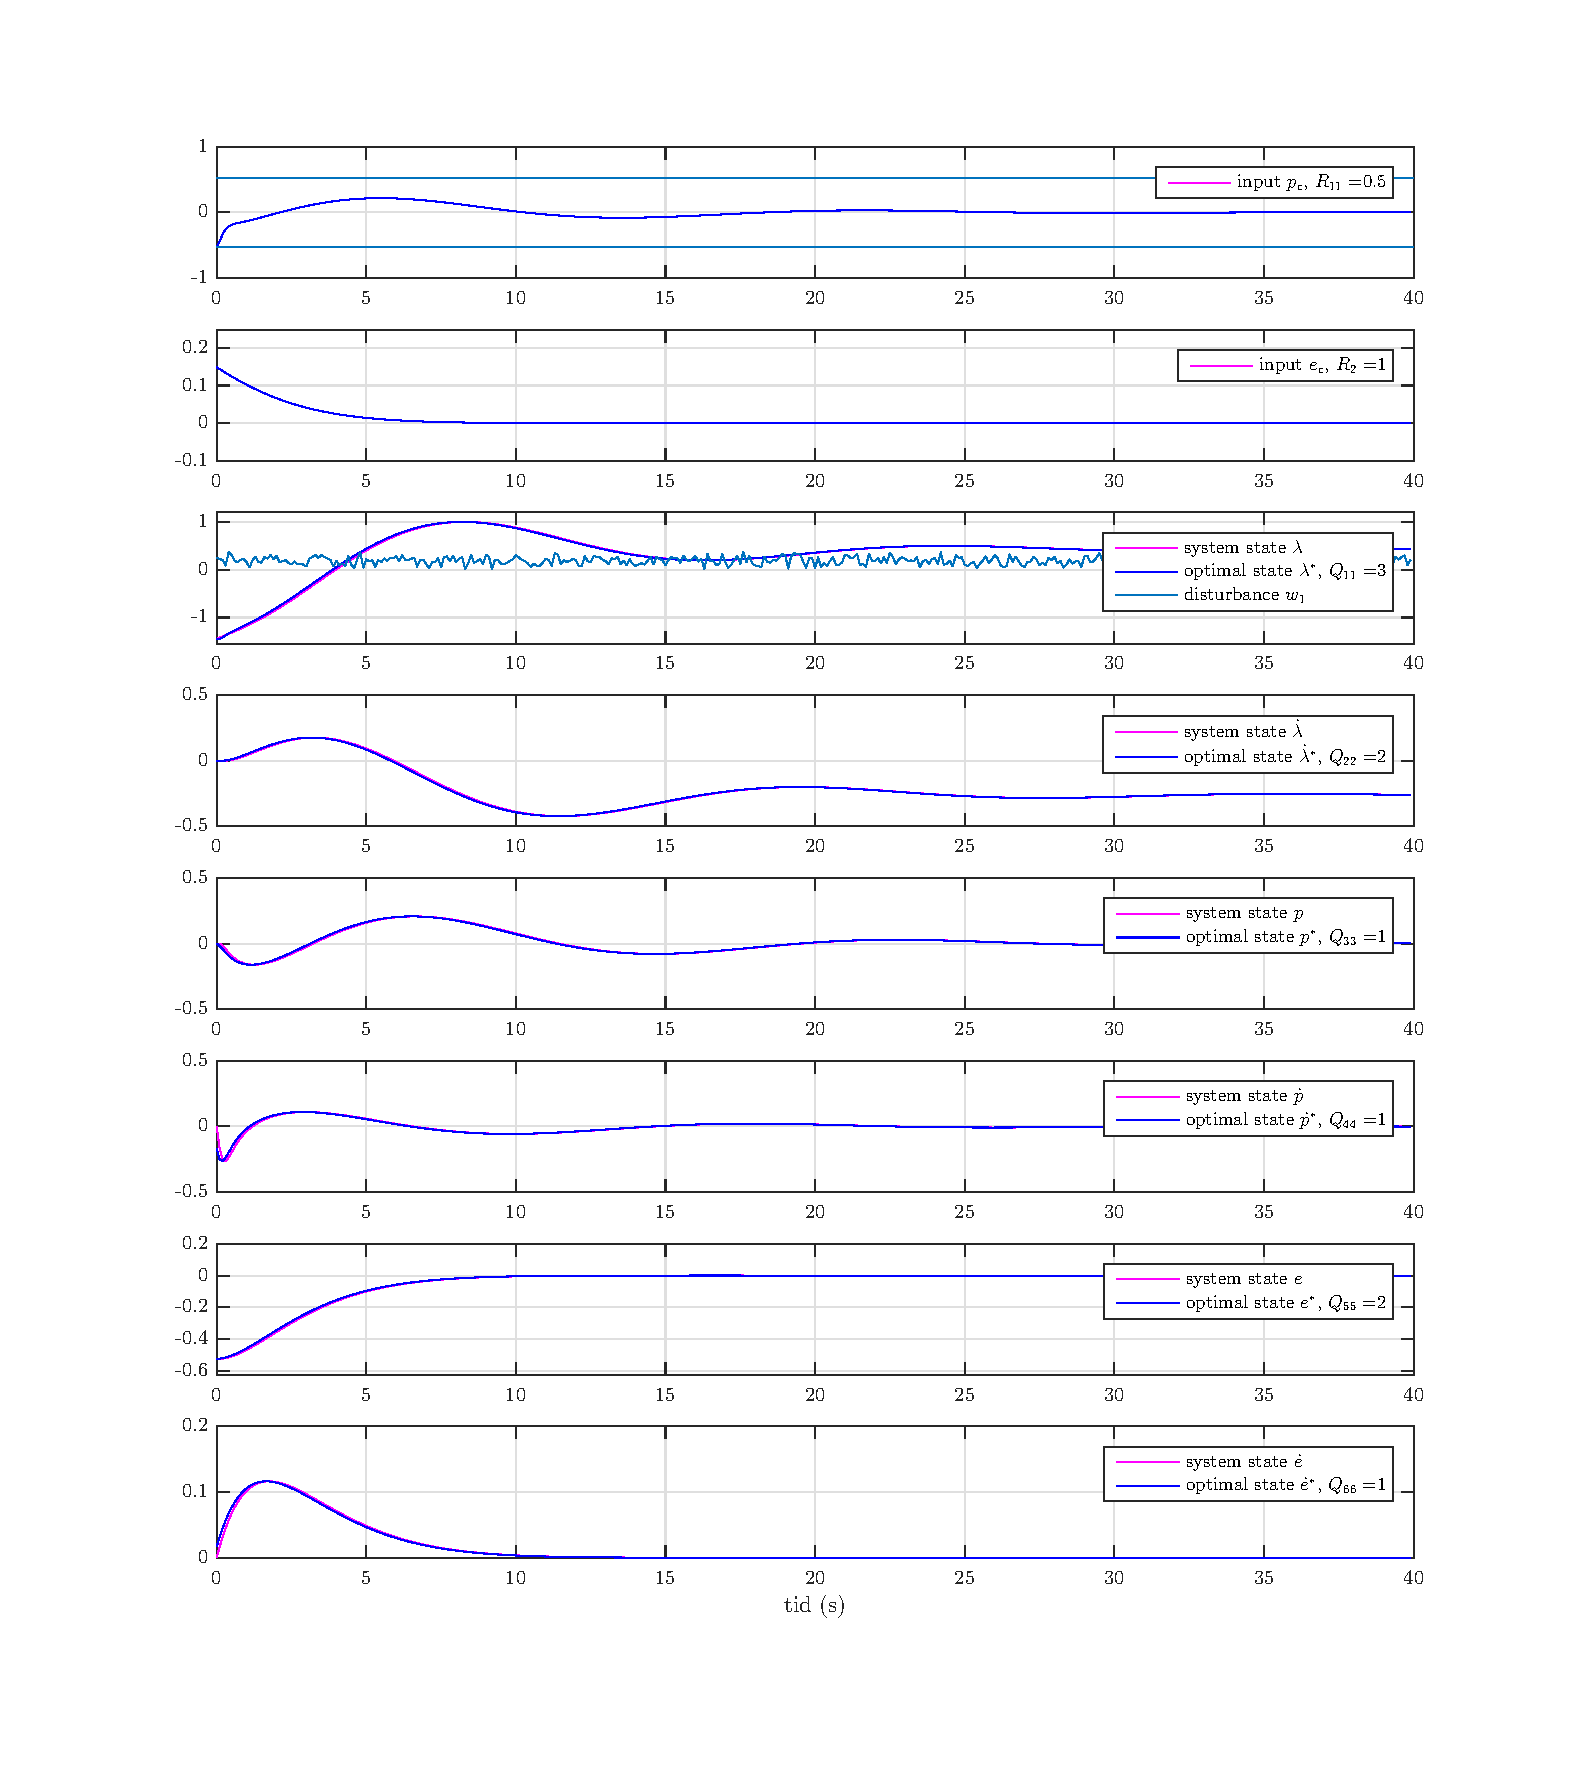
\includegraphics[scale=0.4]{fig/heli_sim_est_not_stable_extended_horizon.eps}
    \caption{Simulation in MATLAB with nominal \acrshort{mpc} and estimator}
    \label{fig:my_label}
\end{figure}

The travel $\lambda$, after 30 seconds, varies between $[0.3752, 0.4175]$. 

A plot of the error dynamics of the estimator is also shown, in addition to the estimator disturbance.

\begin{figure}[h!]
    \centering
    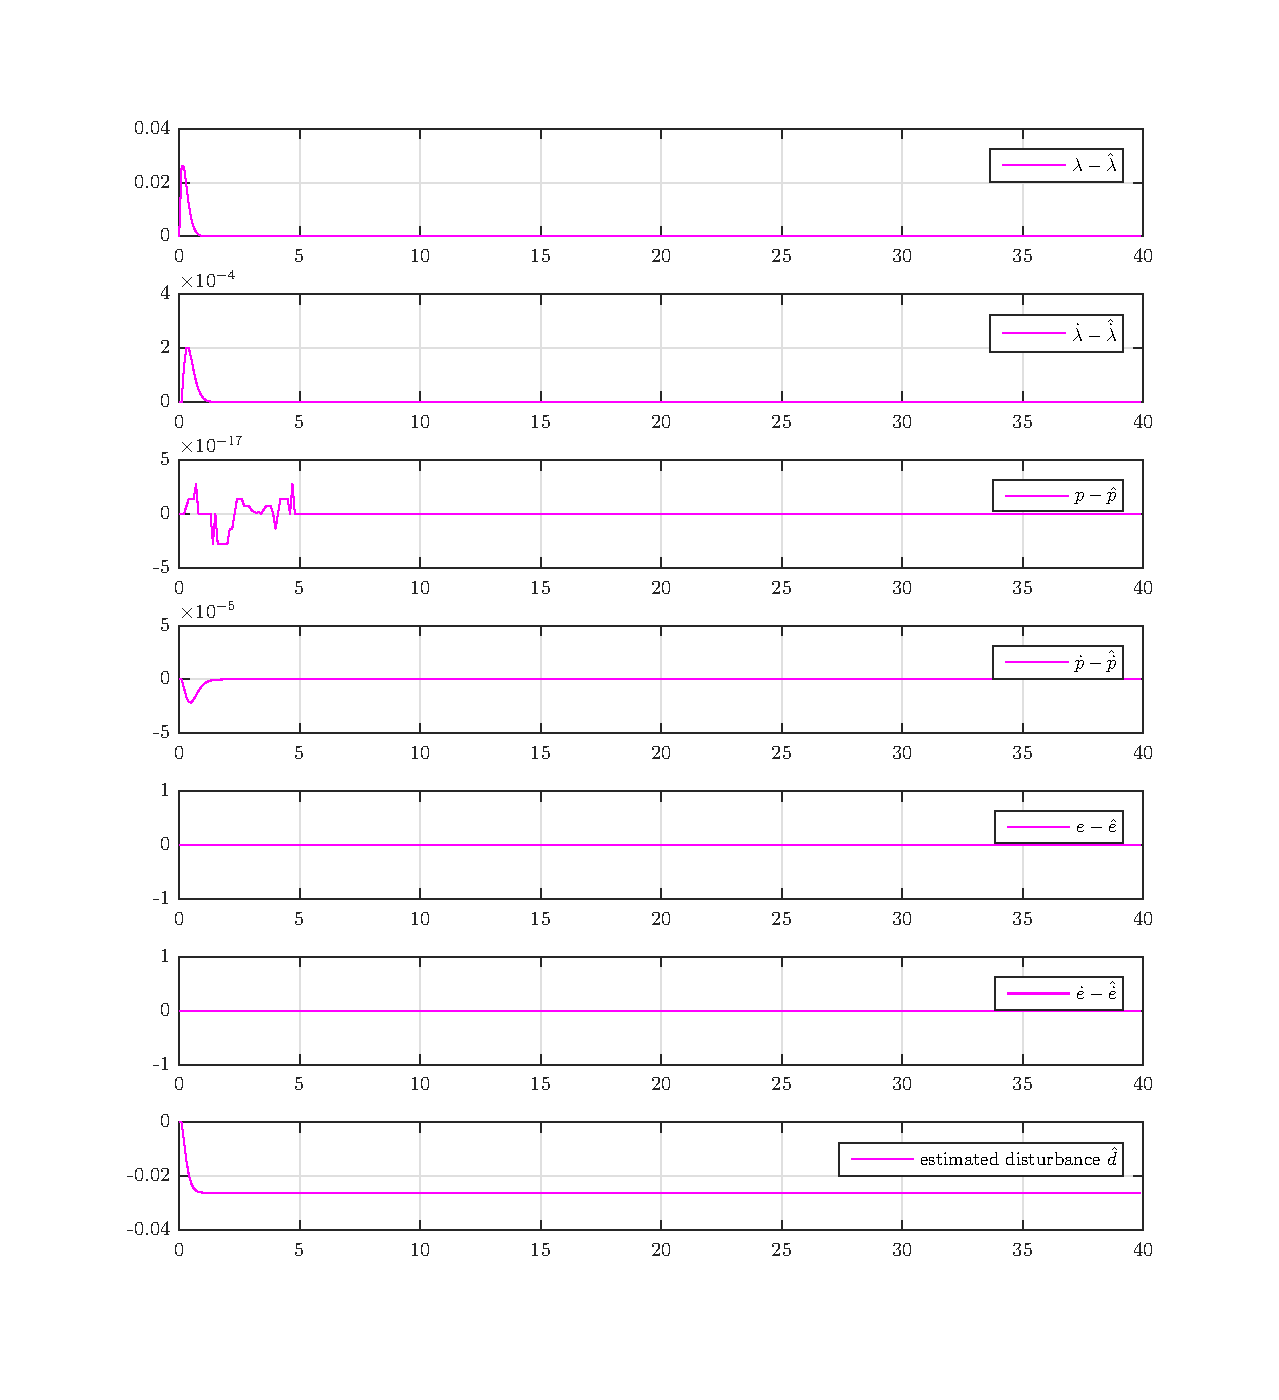
\includegraphics[scale=0.5]{fig/heli_sim_est_not_stable_extended_horizon_error_plot.eps}
    \caption{Error dynamics of estimator with nominal \acrshort{mpc}}
    \label{fig:my_label}
\end{figure}

Now, a terminal constraint and a terminal cost is added to the \acrshort{mpc}. These are described in section \ref{sec:MPC}. 

Firstly, the simulation without an estimator.

The simulation time is halved, because the helicopter tends towards the equilibrium point much faster. 

\begin{figure}[h!]
    \centering
    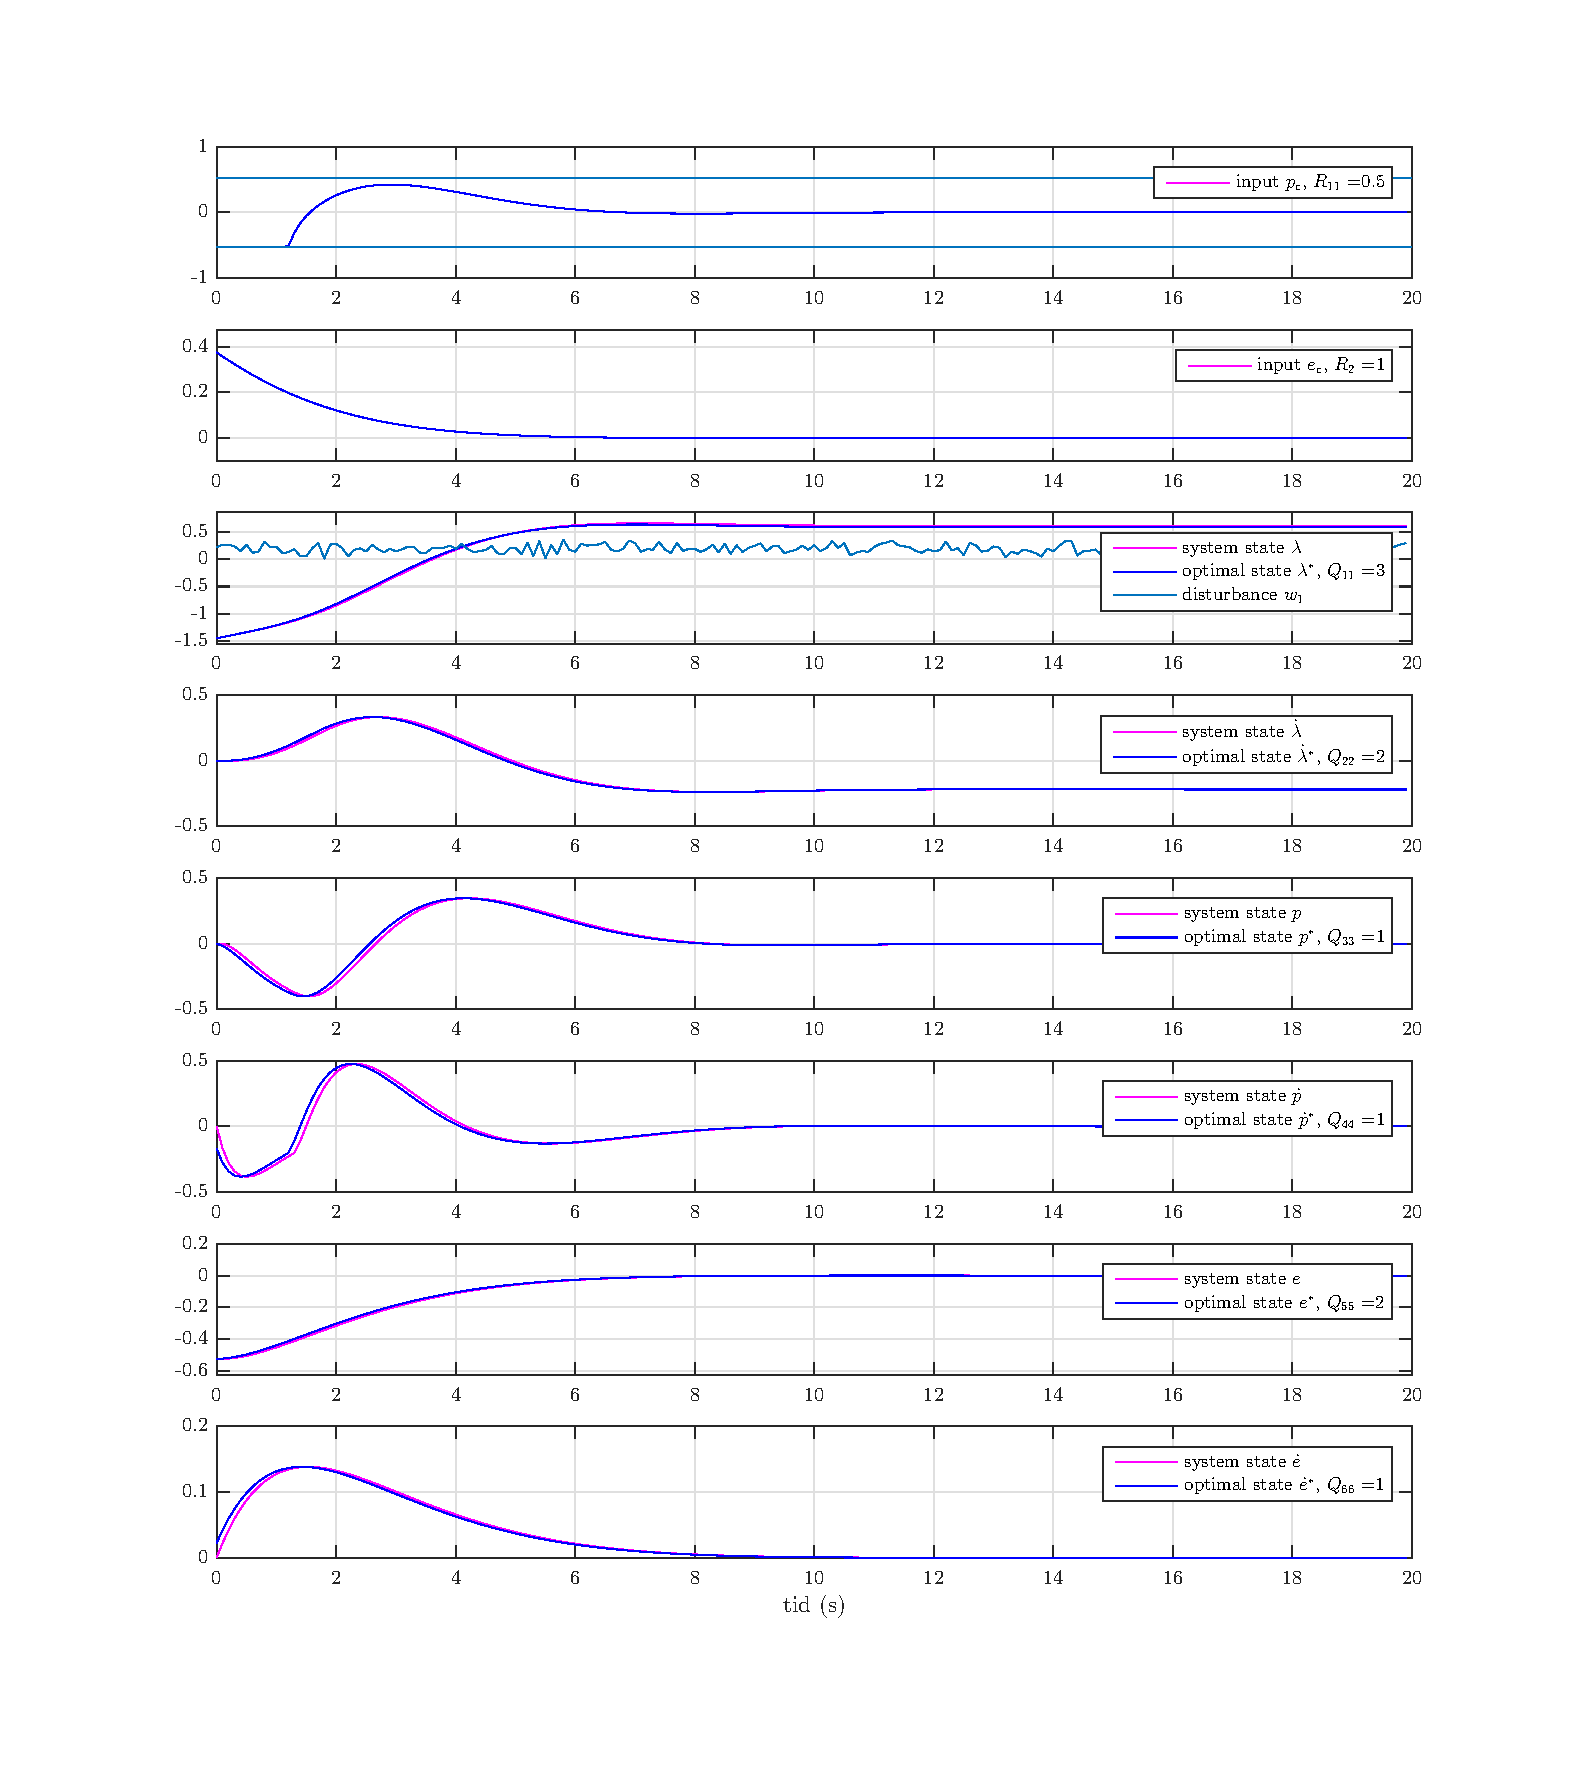
\includegraphics[scale=0.4]{fig/heli_sim_no_est_stable.eps}
    \caption{Simulation in MATLAB with stable \acrshort{mpc}}
    \label{fig:my_label}
\end{figure}

The value of $\lambda$ after 15 seconds, tends towards $[0.6133, 0.6137]$.


Then the same simulation and \acrshort{mpc}, but with an estimator to estimate the constant disturbance to remove the deviation in travel.

\begin{figure}[h!]
    \centering
    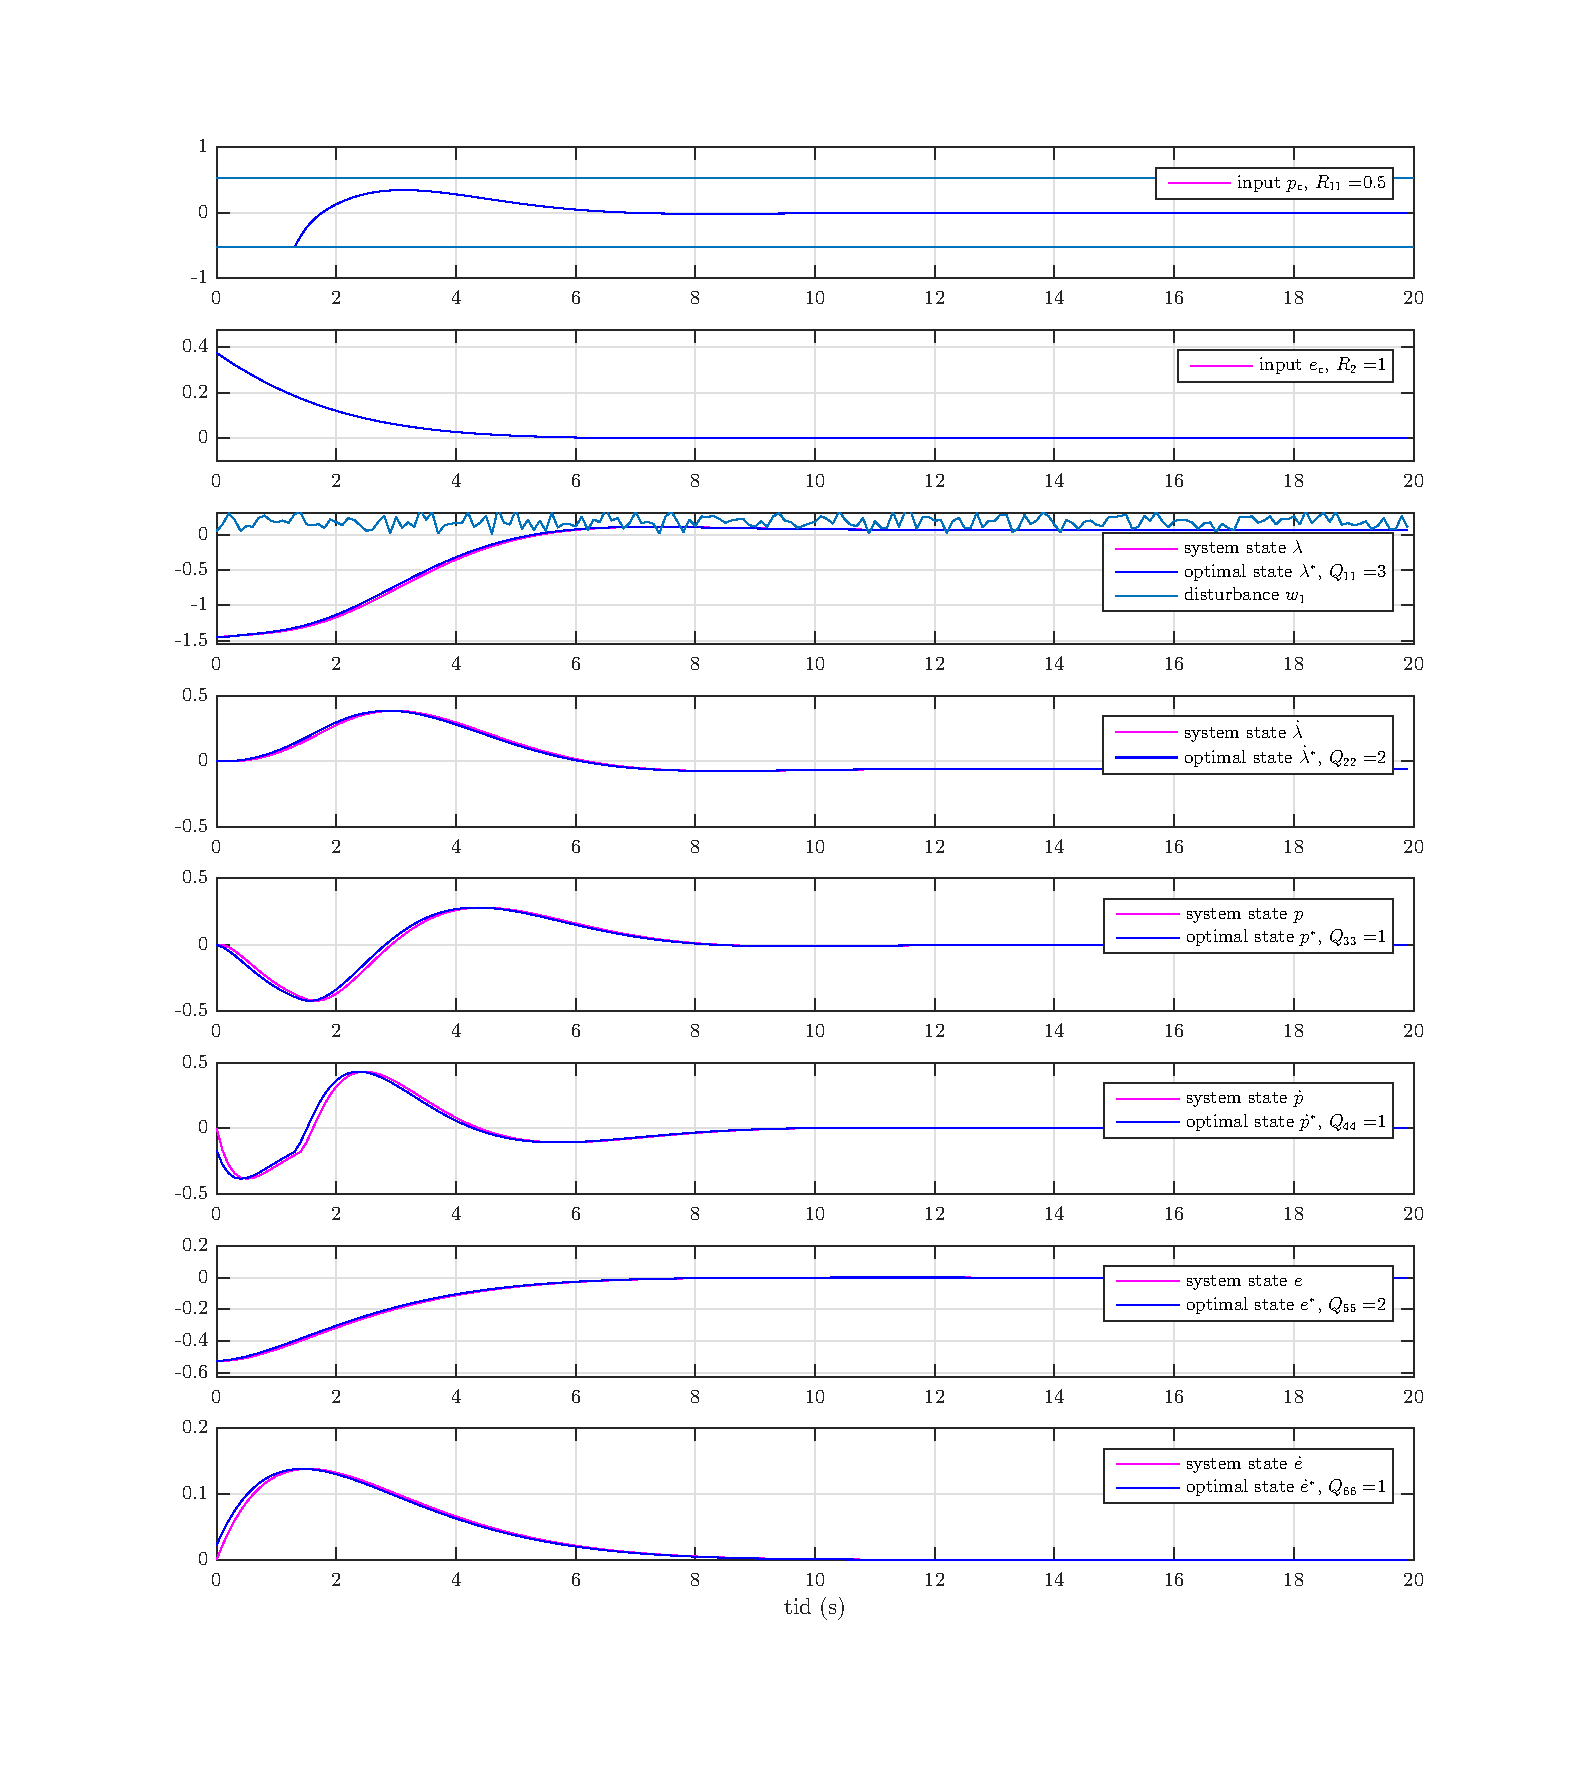
\includegraphics[scale=0.4]{fig/heli_sim_est_stable.eps}
    \caption{Simulation in MATLAB with stable \acrshort{mpc}}
    \label{fig:my_label}
\end{figure}

The value of $\lambda$ tends towards $[0.079]$.

%0.0787, 0.0791

Below is a plot of the error dynamics of the estimator, as well as the estimated disturbance $d$. 

\begin{figure}[h!]
    \centering
    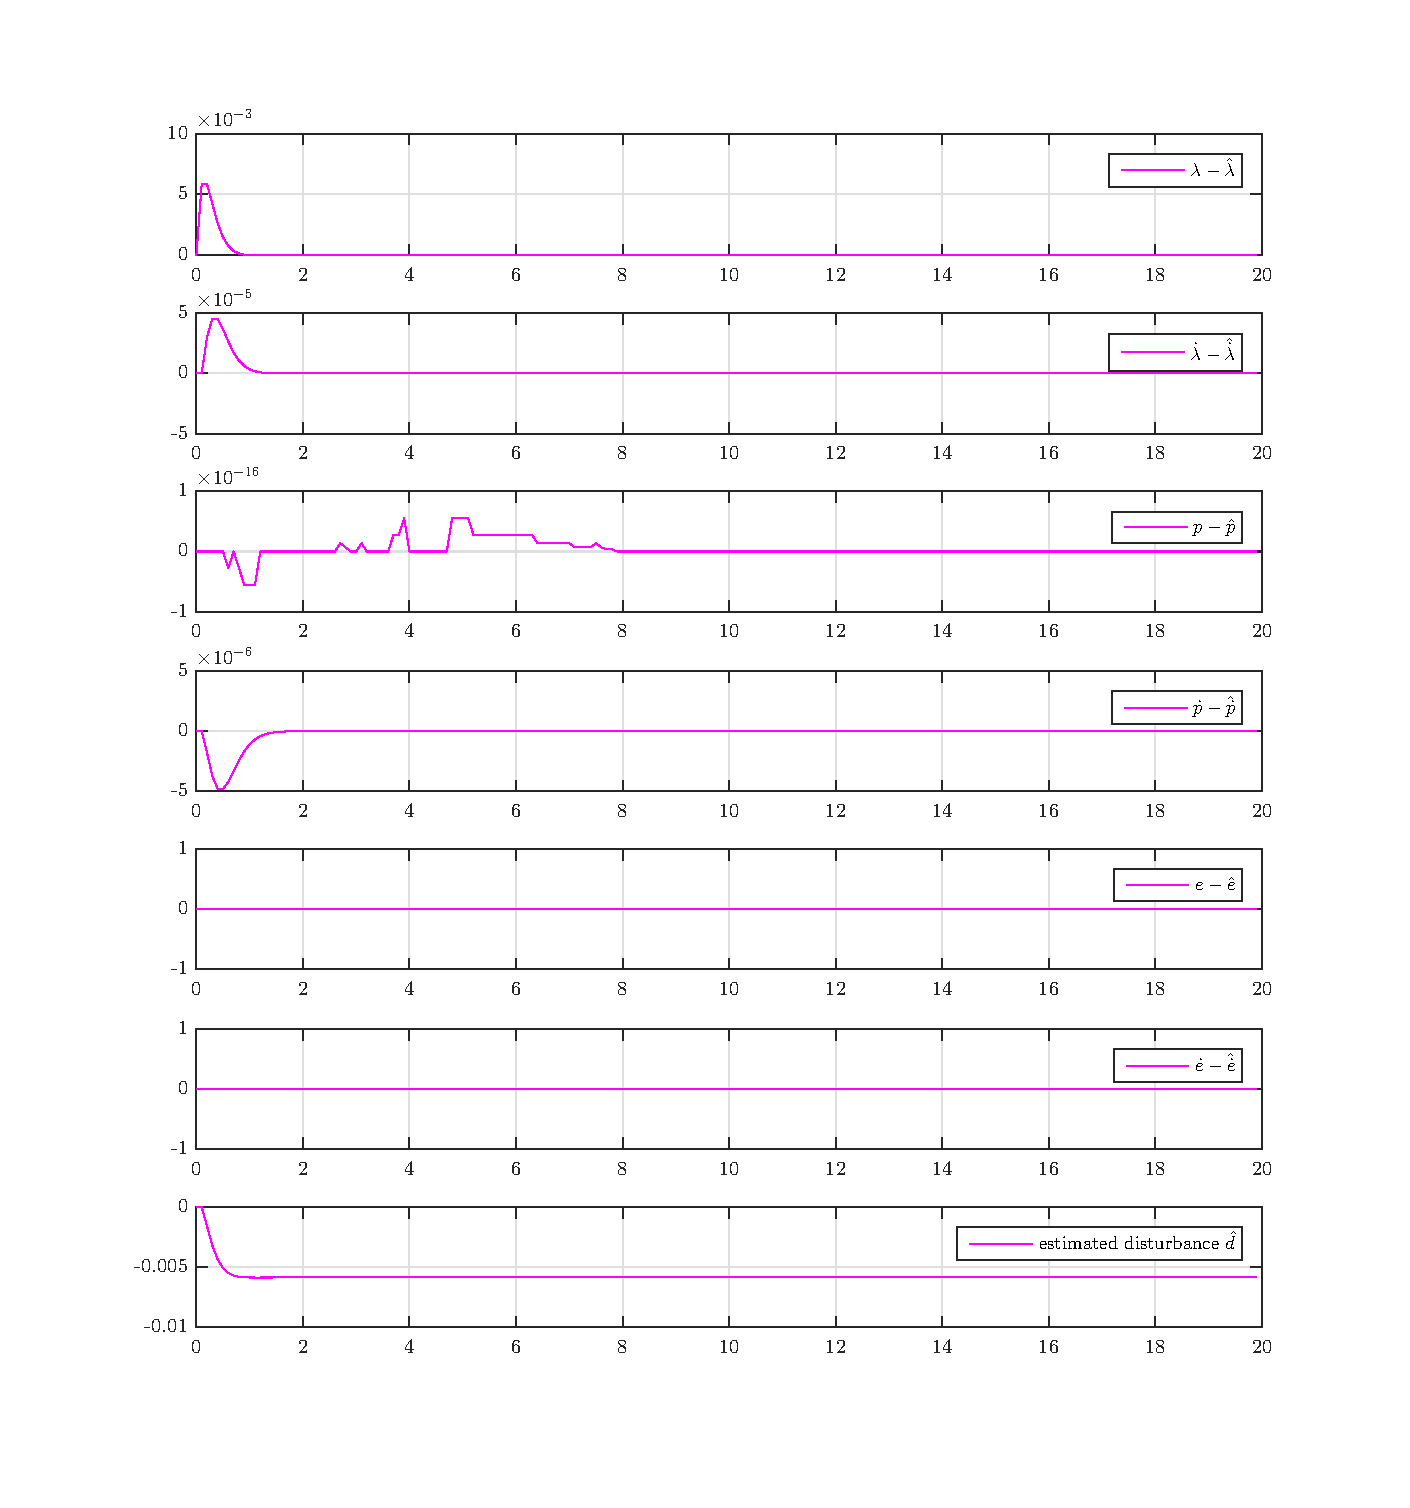
\includegraphics[scale=0.5]{fig/heli_sim_est_stable_error_plot.eps}
    \caption{Error dynamics of stable \acrshort{mpc}}
    \label{fig:my_label}
\end{figure}



\section{Helicopter performance in real time }



Both stable \acrshort{mpc} and unstable \acrshort{mpc}

And no offset as well

This section will demonstrate the effect the frequency of the \acrshort{mpc} has on the performance of the system, and how the frequency was selected. 

What factors come in to play when choosing the optimal frequency for the \acrshort{mpc} to run at.

The model will be run with a frequency of 12.5 Hz, 10 Hz and 5 Hz while the rest of the system will remain on 50 Hz. 

The optimization horizon is 15 in all of these. 
 intervals. 

\begin{figure}
    \centering
    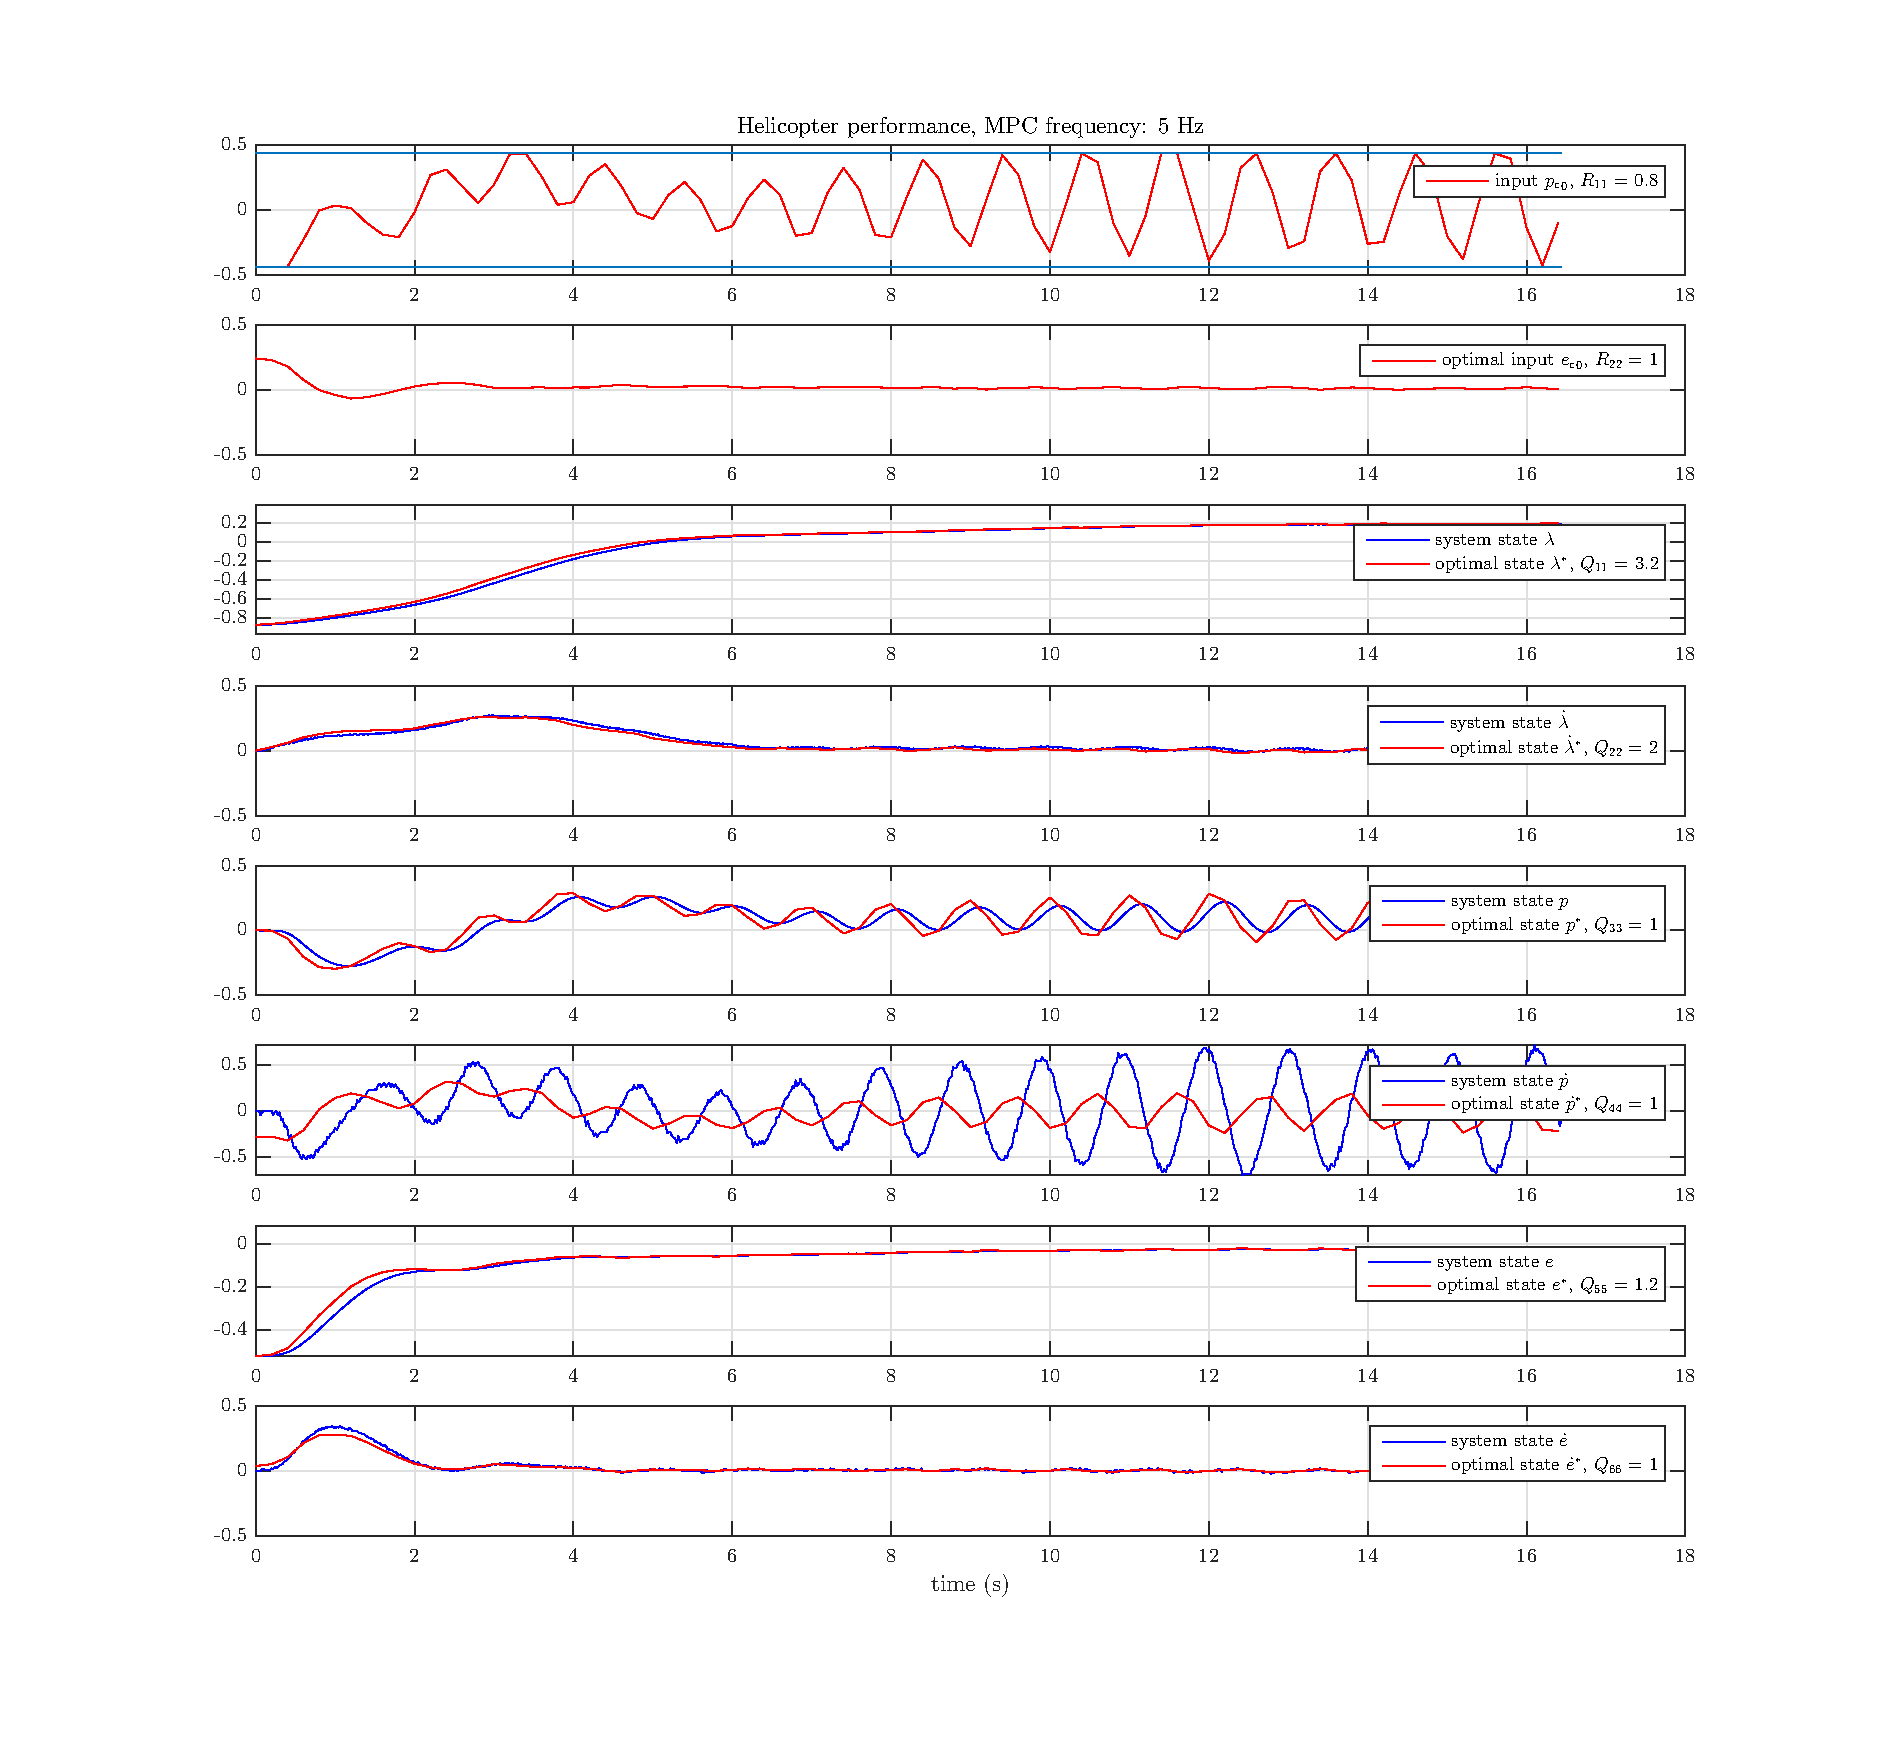
\includegraphics[scale=0.43]{fig/heli_sim_5_15_tune_2.eps}
    \caption{Helicopter performance with \acrshort{mpc} frequency 5 Hz}
    \label{fig:heli_sim_5_1}
\end{figure}


\begin{figure}
    \centering
    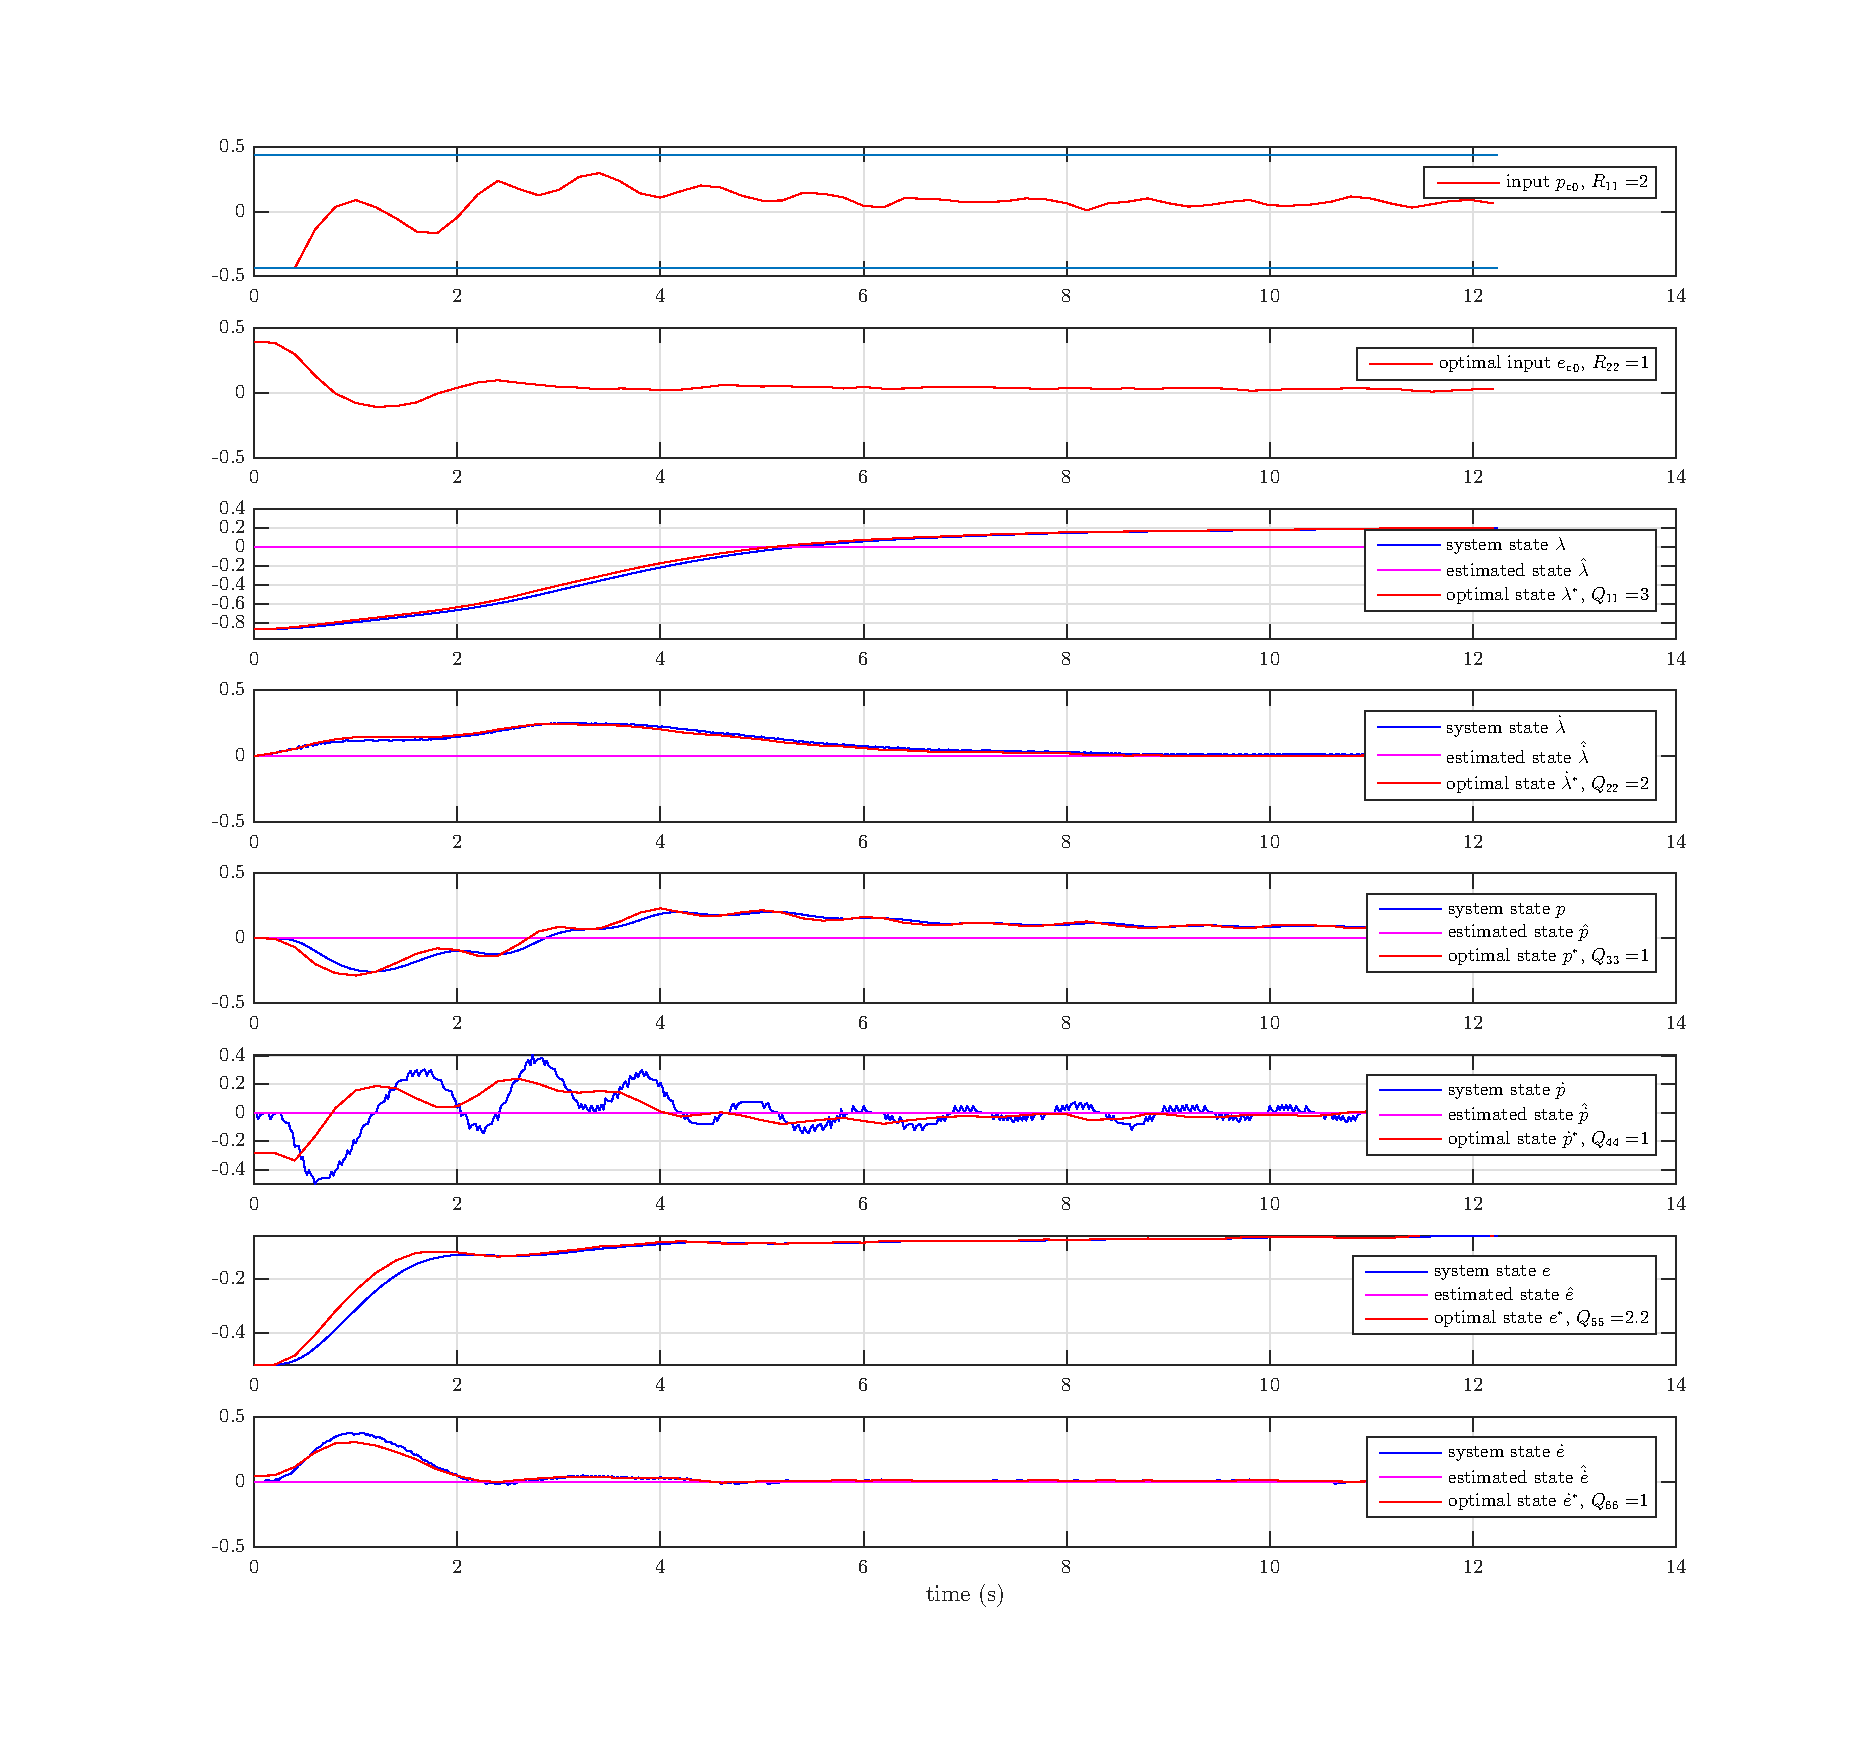
\includegraphics[scale=0.43]{fig/heli_sim_5_15.eps}
    \caption{Helicopter performance with \acrshort{mpc} frequency 5 Hz}
    \label{fig:heli_sim_5_2}
\end{figure}

\begin{figure}
    \centering
    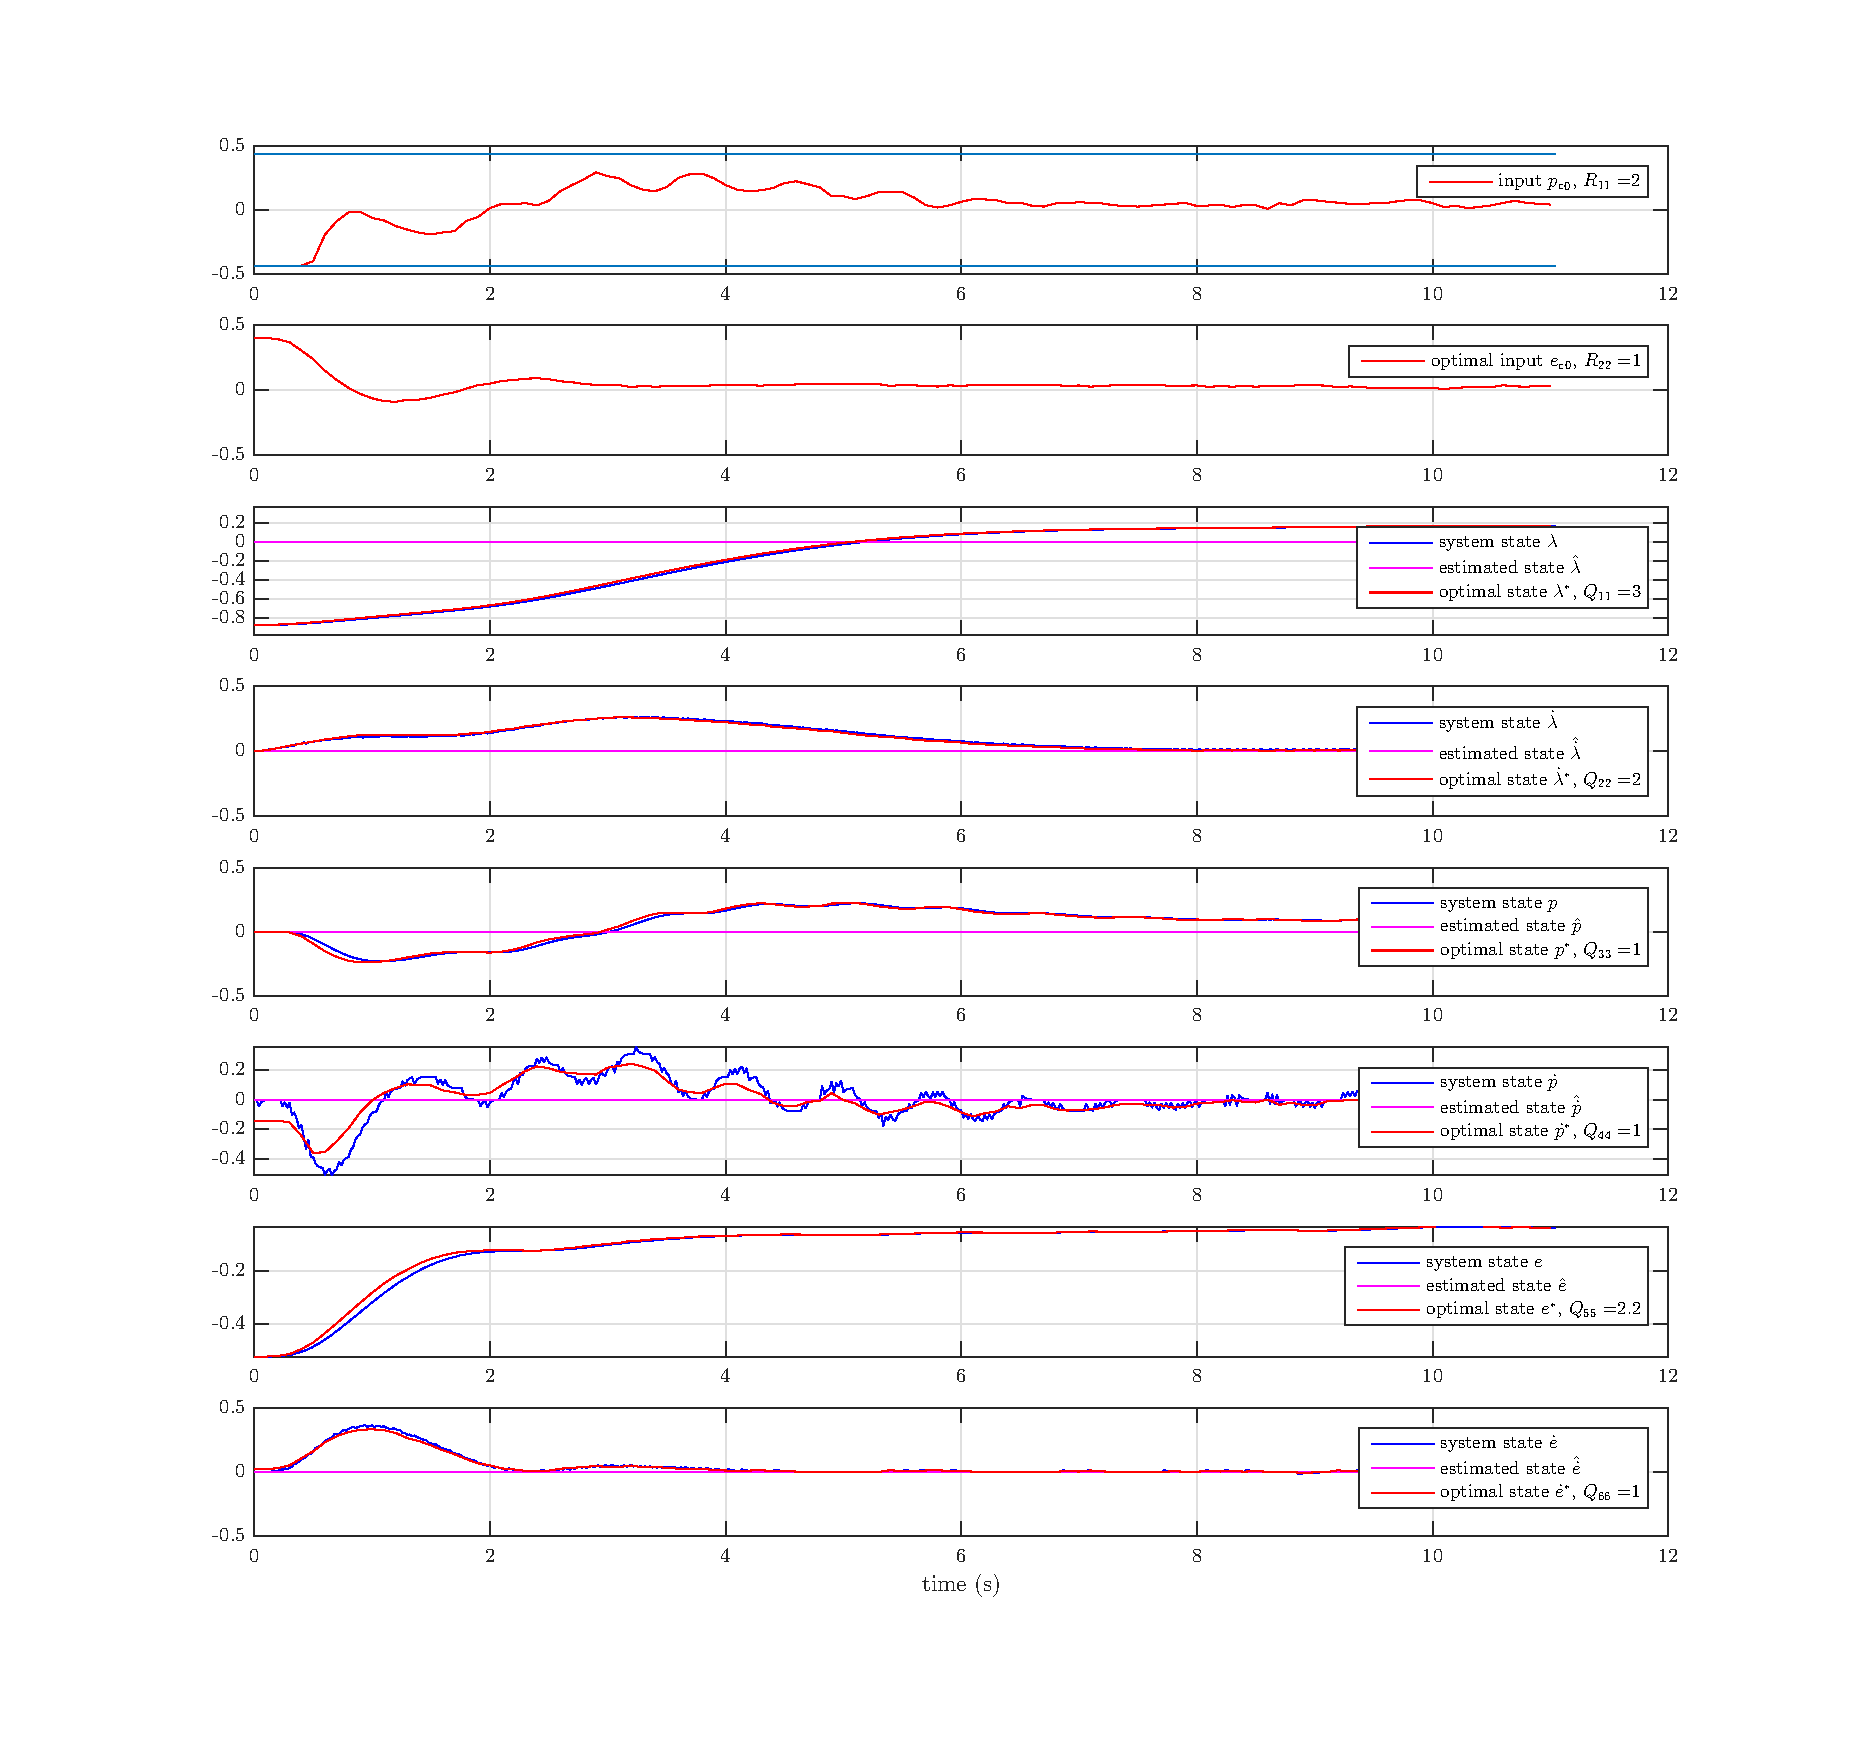
\includegraphics[scale=0.43]{fig/heli_sim_10_15.eps}
    \caption{Helicopter performance with \acrshort{mpc} frequency 10 Hz}
    \label{fig:heli_sim_10_1}
\end{figure}

\begin{figure}
    \centering
    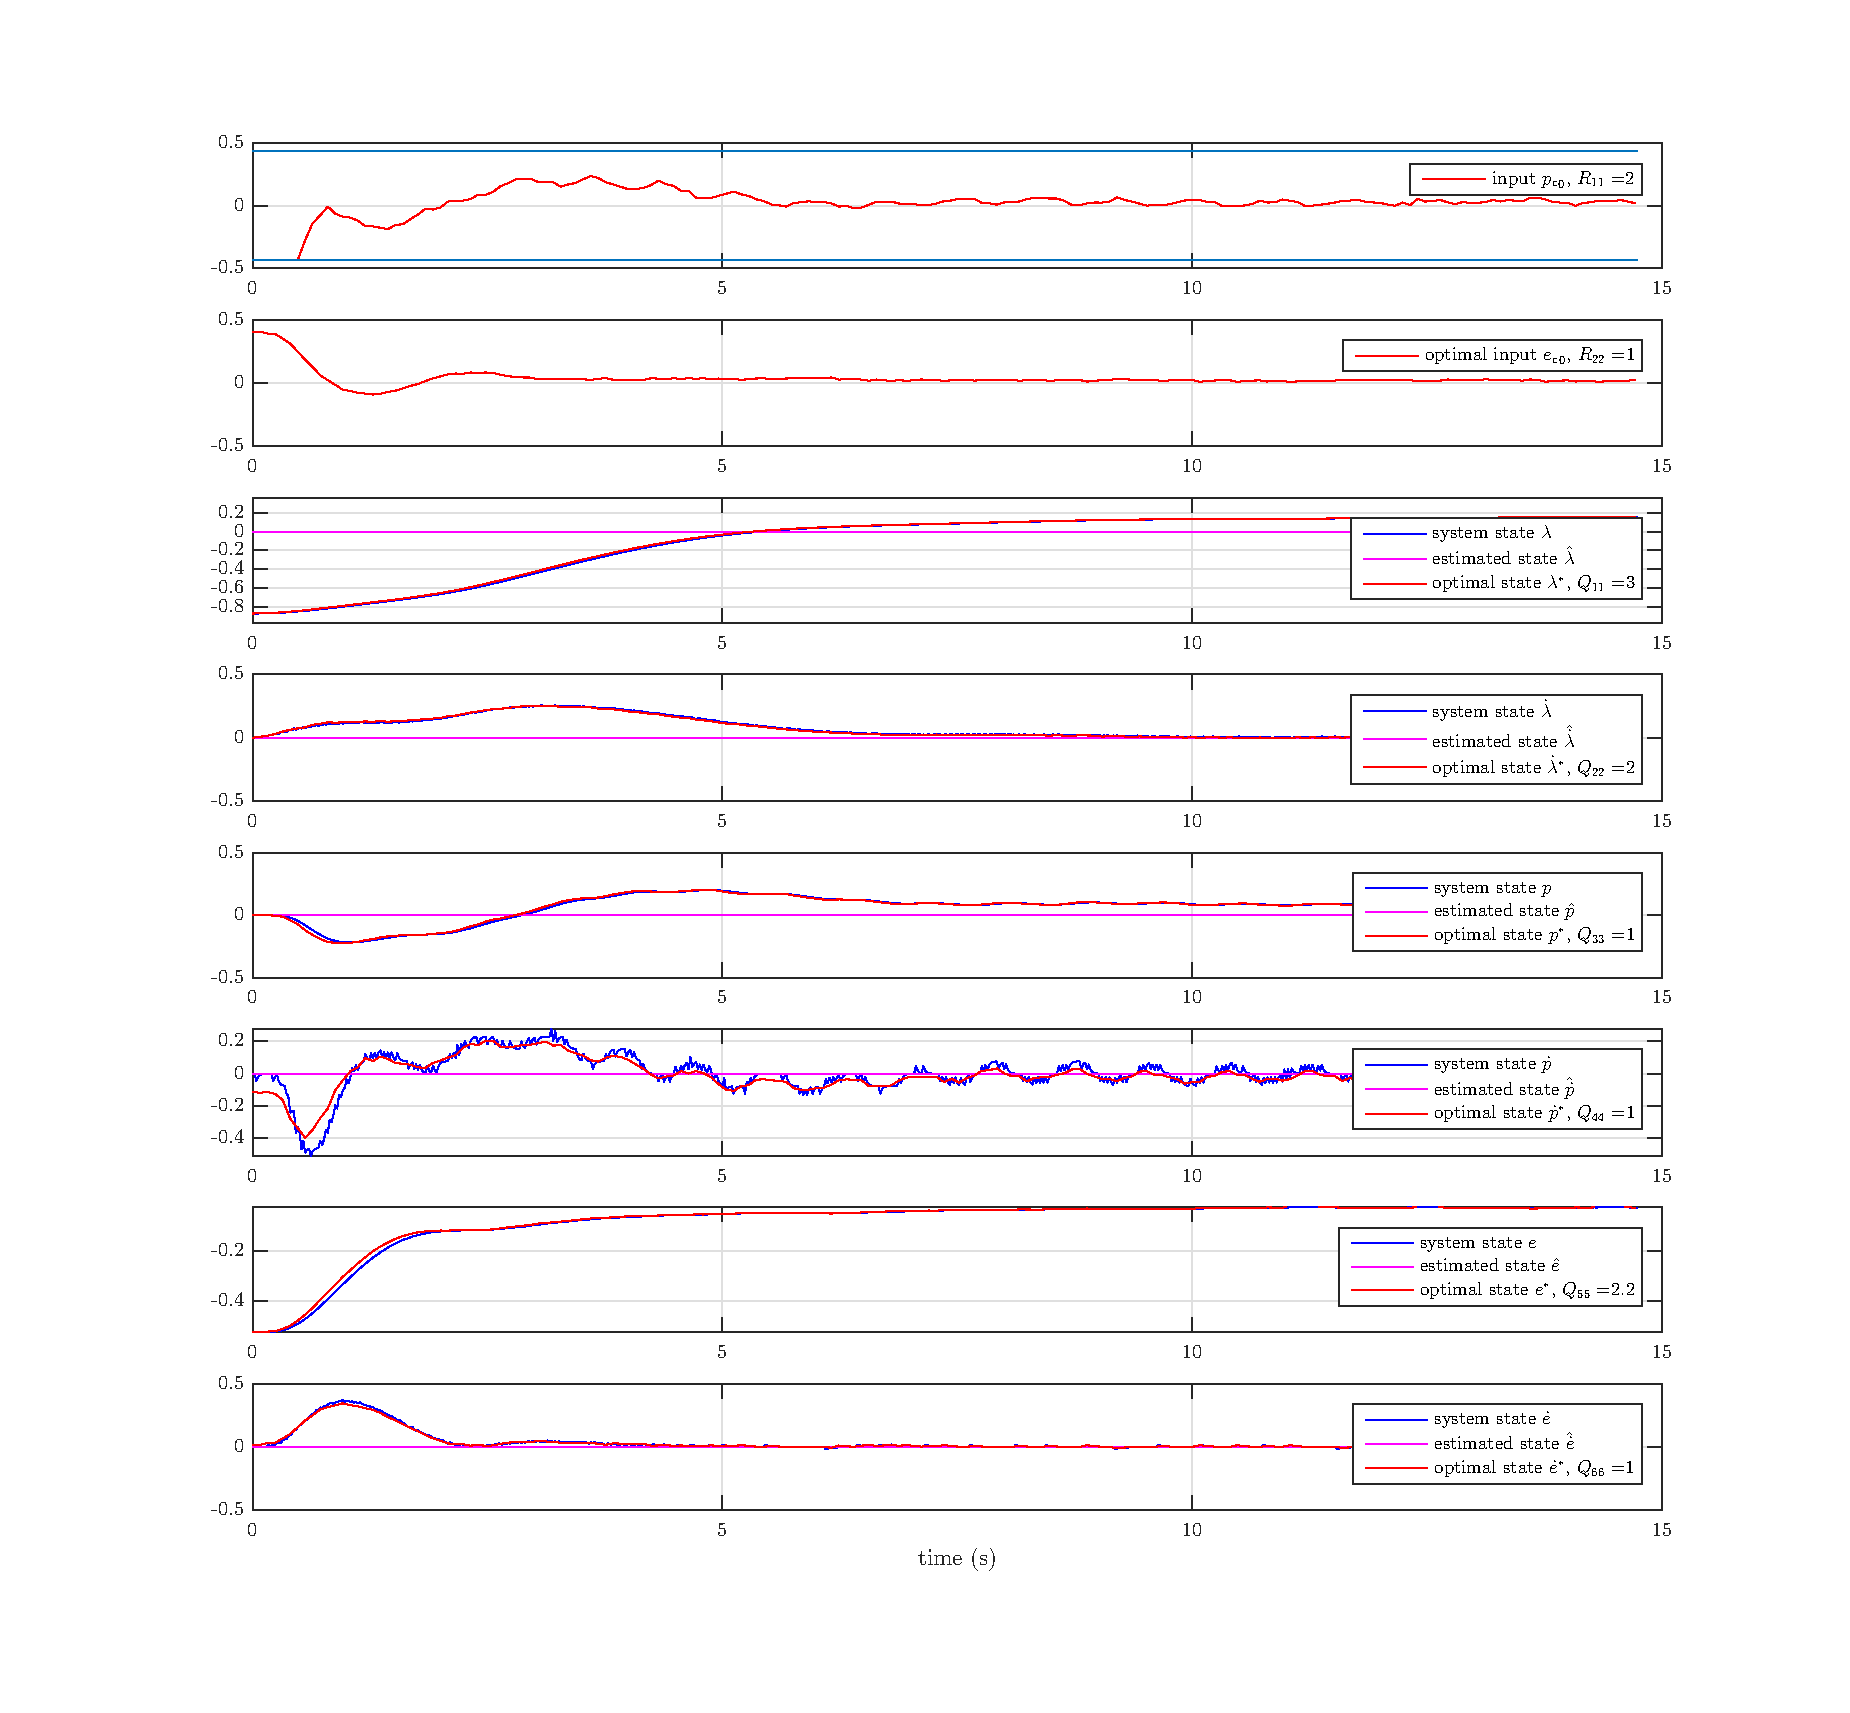
\includegraphics[scale=0.43]{fig/heli_sim_125_15.eps}
    \caption{Helicopter performance with \acrshort{mpc} frequency 12.5 Hz}
    \label{fig:heli_sim_125_1}
\end{figure}

\begin{figure}
    \centering
    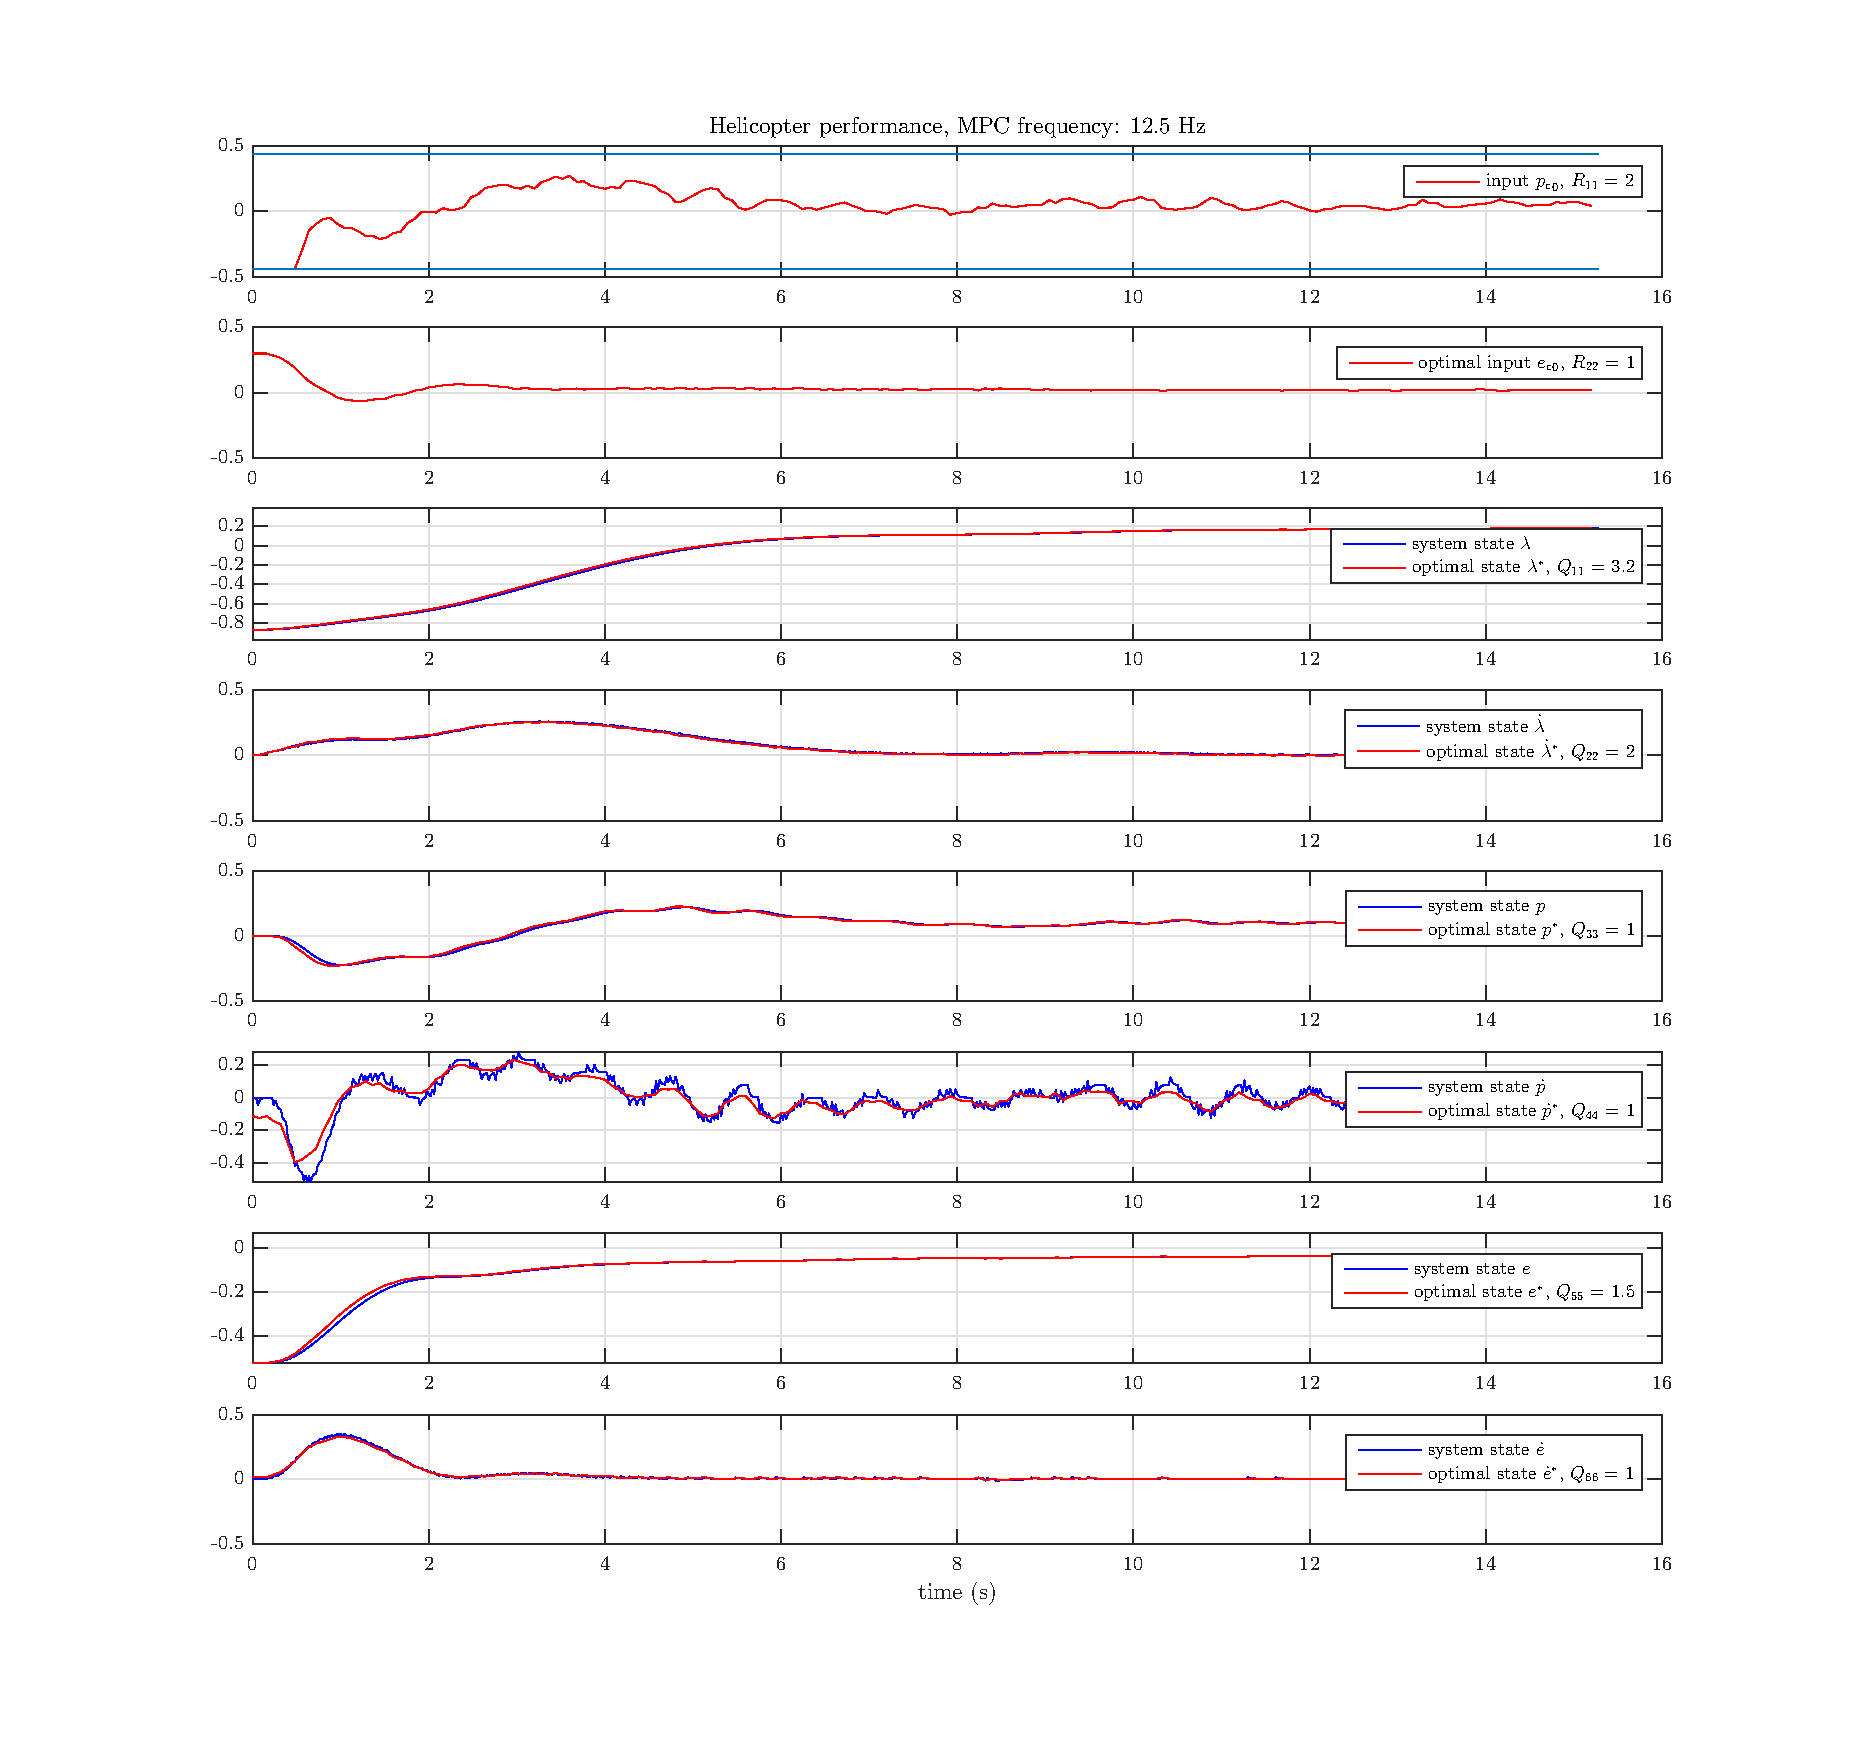
\includegraphics[scale=0.43]{fig/heli_sim_125_15_tune_3.eps}
    \caption{Helicopter performance with \acrshort{mpc} frequency 12.5 Hz}
    \label{fig:heli_sim_125_2}
\end{figure}


\section{OSQP performance}




